
%%\documentclass[referee,sn-basic]{sn-jnl}% referee option is meant for double line spacing

%%=======================================================%%
%% to print line numbers in the margin use lineno option %%
%%=======================================================%%

%%\documentclass[lineno,pdflatex,sn-basic]{sn-jnl}% Basic Springer Nature Reference Style/Chemistry Reference Style


%\documentclass[pdflatex,sn-mathphys-num]{sn-jnl}% Math and Physical Sciences Numbered Reference Style
%%\documentclass[pdflatex,sn-mathphys-ay]{sn-jnl}% Math and Physical Sciences Author Year Reference Style
%%\documentclass[pdflatex,sn-aps]{sn-jnl}% American Physical Society (APS) Reference Style
%%\documentclass[pdflatex,sn-vancouver-num]{sn-jnl}% Vancouver Numbered Reference Style
%%\documentclass[pdflatex,sn-vancouver-ay]{sn-jnl}% Vancouver Author Year Reference Style
\documentclass[pdflatex,sn-apa]{sn-jnl}% APA Reference Style
%%\documentclass[pdflatex,sn-chicago]{sn-jnl}% Chicago-based Humanities Reference Style

%%%% Standard Packages
%%<additional latex packages if required can be included here>

\usepackage{graphicx}%
\usepackage{multirow}%
\usepackage{amsmath,amssymb,amsfonts}%
\usepackage{amsthm}%
\usepackage{mathrsfs}%
\usepackage[title]{appendix}%
\usepackage{xcolor}%
\usepackage{textcomp}%
\usepackage{manyfoot}%
\usepackage{booktabs}%
\usepackage{algorithm}%
\usepackage{algorithmicx}%
\usepackage{algpseudocode}%
\usepackage{listings}%
\usepackage{tikz}
\usetikzlibrary{shapes.geometric, arrows.meta, positioning, calc}
%%%%

\raggedbottom
%%\unnumbered% uncomment this for unnumbered level heads

\begin{document}

\title[AI Disaster Opinions and Action]{Breaking the Bubble? AI’s Role in Shaping Disaster Opinions and Driving Social Action}

%%=============================================================%%
%% GivenName	-> \fnm{Joergen W.}
%% Particle	-> \spfx{van der} -> surname prefix
%% FamilyName	-> \sur{Ploeg}
%% Suffix	-> \sfx{IV}
%% \author*[1,2]{\fnm{Joergen W.} \spfx{van der} \sur{Ploeg} 
%%  \sfx{IV}}\email{iauthor@gmail.com}
%%=============================================================%%

\author*[1, 2]{\fnm{Tina} \sur{Comes}}\email{t.comes@tudelft.nl}

\affil*[1]{\orgdiv{Faculty Technology, Policy \& Management}, \orgname{TU Delft}, \orgaddress{ \city{Delft}, \country{The Netherlands}}}

\affil[2]{\orgdiv{Institut for the Protection of Terrestrial Infrastructures}, \orgname{DLR}, \orgaddress{ \city{Sankt Augustin}, \country{Germany}}}

%%==================================%%
%% Sample for unstructured abstract %%
%%==================================%%

\abstract{Crises change human information collection, sharing, and decision-making. The combination of urgency, uncertainty, and high-stakes is known to induce cognitive biases, informational bubbles and echo chambers. Trustworthy Artificial Intelligence (AI) promises solutions to optimise decisions and reduce informational bottlenecks. Yet, introducing AI as a 'trusted' actor in crises fundamentally changes human interaction, information processing and decision-making. While the literature on Human-Centred AI often focuses on the impact of an AI on individual biases or decisions, what is missing is an understanding at scale how AI shapes information processing, opinions and decisions during volatile and uncertain conditions as typical for disasters.

This paper uses an agent-based model (ABM) to explore how AI impacts information processing, sharing and decision-making during crises, especially if that AI seeks to gain trust by tuning into human beliefs. To explore the effects for different prototypical behaviours, the human agents in the ABM adopt exploratory or exploitative behaviours modelled through Q-learning algorithms and update their beliefs using Bayesian techniques. 

Our findings reveal nuanced interactions: AI can initially improve situational awareness, it often inadvertently introduces or reinforces new echo chambers and interrupts social networks. Identifying tipping points where AI transitions from mitigating to amplifying filter bubbles provides critical insights to understand how to balance use of AI and accuracy, and how much inaccuracy might be needed.}

\keywords{Disaster Response, AI for Good, Opinion Dynamics, Filter Bubble, Echo Chamber, Opinion-Action Dynamic, Hybrid Intelligence}

%%\pacs[JEL Classification]{D8, H51}

%%\pacs[MSC Classification]{35A01, 65L10, 65L12, 65L20, 65L70}

\maketitle

\section{Introduction}\label{sec1}
Increasingly, we humans rely on artificial intelligence (AI) to collect and analyse information and make decisions \citep{klingbeil2024trust}. This trend is particularly pronounced during crises, where decision-makers are confronted with highly complex decisions that need to be addressed urgently, leaving limited time for reflection and deliberation \citep{mendonca2001decision}. This combination is known to deeply impact human information processing, sharing decision-making behaviour \citep{comes2020coordination}. To help humans manage this complexity, Artificial Intelligence (AI) is promoted as a tool to optimise decisions and information flows \citep{jeon2024hearhere}. The idea that AI will facilitate immediate access to "objective', 'data-driven' or neutral information, or facilitate interaction with diverse viewpoints is expected to improve situational awareness and prevent fragmentation. 

A prerequisite to the use of technology in crises is trust \citep{steinbrink2024impact}. In the field of AI, there is a plethora of guidelines and approaches that speak to designing AI that is \textit{trustworthy}, especially in the context of crises and disasters. For a recent review, see \citep{albahri2024systematic}. Often, the trust relationship is conceptualised as one individual trusting one AI, whereby it is claimed that trust is promoted by more transparency \citep{visave2025transparency}. Others focus on \textit{public} trust as a result of a design and decision-making process \citep{tzachor2020artificial}. Recognising that humans, especially in crises, have a tendency of selective exposure \citep{barbera2015tweeting} and confirmation bias \citep{paulus2024interplay}, whereby they reject conflicting information. 

Increasingly, generative AI (genAI) has started to mimic human behaviour and tune to the opinions of humans \citep{sharma2024generative} as a way to gain acceptance and 'trust'. This introduces a dilemma: should AI provide accurate information, even if it contradicts beliefs and is potentially rejected, or should it align with human beliefs to foster acceptance and trust? If AI overly tunes into existing beliefs to gain rapid trust, it risks amplifying cognitive biases and echo chambers \citep{ekstrom2022self}. Echo chambers are segregated information spaces, in which pre-existing beliefs are reinforced, and there is limited exposure to diverse or contradictory perspectives \citep{jeon2024hearhere}. Echo chambers have been linked to polarisation, or increasing discord between different groups and communities \citep{interian2023network}. This is highly problematic in crises, since social coherence is a cornerstone of (community) resilience and efficient response \citep{champlin2023measuring}. 

While studies and insights on the implications of genAI models for human trust and decision-making have started to emerge \citep{zhang2024see, sharma2024generative}, a gap in current research is understanding how the interactions of individuals with AI scale up to communities and broader (social) networks during crises, potentially creating or exacerbating echo chambers and polarisation. This paper addresses this gap by investigating the social and networked aspects of AI and exploring if and in how far AI can act as a bridge that connects communities by providing broader perspectives during crises, or if it instead reinforces echo chambers through alignment with prior beliefs intended to gain acceptance and break into prior beliefs. Since these questions are essentially about alignment tipping points and the rise or collapse of echo chambers, I use here the rich literature from resilience theory \citep{folke2016resilience} to describe the emergence, dynamics and potential collapse or perseverence of echo chambers. In essence, a tipping point describes a qualitative change in a system described mathematically as a bifurcation \citep{milkoreit2018defining}.

To start exploring these tipping point dynamics, we lean on complexity science and use an agent-based modelling (ABM) approach that allows us to simulate interactions between heterogeneous human agents and AI during crises. The model simulates decentralised disaster relief efforts where human agents, characterised by distinct behavioural types, interact with human or AI information sources to allocate resources across a spatial environment. This approach enables us to observe emergent patterns of information acquisition; belief formation and updating; and decision outcomes across different networks, environments and behavioural strategies. We analyse the implications of different alignment levels on the adoption of AI, and the resulting social or AI-driven echo chambers, situation awareness and decision performance. 

Information acquisition by agents is modelled through a Q-learning mechanism that determines the sources queried, enabling dynamic belief revision based on delayed evidence from the assistance delivered. To model information acceptance and belief updates, the model adopts established opinion dynamics frameworks \citep{geschke2019triple}, but seeks to understand the impact of different human behavioural patterns and biases. To this end, we analyse two different prototypical human decision-making strategies under uncertainty as a way to manage the trade-off between broad information collection to reduce uncertainty (exploration) and reward seeking within limited local environments (exploitation) - the latter pattern being typical for the responsive short-term focus of crisis management \citep{comes2020coordination}. 

This approach allows us to analyse how different information sources, behavioural patterns and dynamic trust relationships influence situational awareness and decision-making in dynamic and uncertain networks. The analysis identifies tipping points where the benefits of AI of being able to exploring broader areas transition into detrimental influence that amplifies echo chambers. These insights contribute to the ongoing discussions about what constitutes \textit{trustworthy} versus \textit{trusted} or used AI. 

\section{Background}

Fuelled by climate change, increasing inequalities, conflict and war, we are confronted with global poly-crises that erode progress towards sustainability \citep{sogaard2024evolution}. As crises require rapid interventions that overwhelm human decision-making capacity, digital tools have been portrayed as a potential avenue to automatically collect and analyse data to support or make decisions \citep{qadir2016crisis}. Examples range from community mapping \citep{champlin2023measuring, soden2014crowdsourced}, the use of aerial images, remote sensing, UAVs and digital platforms for better crisis management \citep{voigt2007satellite} to increasing automation of the delivery of aid, facilitated by mobile phone and blockchain technology \citep{coughlan2015forecast, baharmand2019leveraging}. Despite these technological advances, the emergent nature of crises poses challenges for information collection, sharing, and decision-making \citep{turoff2004design, nespeca2020towards}.

To better understand the use of AI in the context of crises, we refer to the information management cycle that distinguishes three mechanisms (i) information collection and verification, (ii) information sharing and dissemination and (iii) information use and decision-making \citep{van2015On}. Table \ref{tab:AIcrisis-overview} provides an overview of the promises and perils of AI for the different information management mechanisms, crucial human behavioural patterns and examples of the use of AI in this context. The following sections examine how AI changes these three mechanisms and underlying social and behavioural structures.

\begin{table}
    \small
    \centering
    \begin{tabular}{p{0.15\textwidth} | p{0.15\textwidth} p{0.17\textwidth}p{0.17\textwidth} p{0.17\textwidth}}
        \hline
        \textbf{Mechanism} & \textbf{Promise of AI} &\textbf{ Peril of AI} & \textbf{Human Behaviour} & \textbf{Example Application}\\ \hline
        Information collection & Real-time large-scale information collection \citep{narmatha2025disaster} & Exclusion of marginalised or digitally invisible groups \citep{coleman2024weaving} & Sensemaking \citep{klein2010rapid} & Crowd sensing \citep{mai2025evaluating}, wild fire monitoring \citep{roy2024multi}\\ \hline
        Information sharing & Facilitate access to diverse sources \citep{jeon2024hearhere} & Sharing confined to closed social networks & Trust and alignment, over-reliance \citep{manzini2024should} & Chatbots \citep{urbanelli2024ermes}\\ \hline
        Decision support &  AI delivering tailored and verified information \citep{zhao2025tailoring}, recommendations, automated decisions & Promoting high alignment \citep{manzini2024should}; (moral) de-skilling \citep{vallor2015moral} & (Group) decisions \citep{comes2024ai}, cognitive biases \citep{paulus2022influence} & Agentic AI \citep{acharya2025agentic}, Early Warning \citep{reichstein2025early}\\ \hline
    \end{tabular}
    \caption{Overview of key mechanisms, promise and perils of AI in crisis management}
    \label{tab:AIcrisis-overview}
\end{table}


\subsection{Information collection: knowing more or knowing better?}
AI in combination with data collection via remote sensing or mobile technologies promises a broader perspective, addressing both network density and information intensity that often lack in human social networks \citep{pan2012crisis}. The promise of real-time data collection, especially in highly dynamic situation, is said to allow decision-makers to identify critical tipping points rapidly, before they occur and crises spiral out of control. For almost two decades, focus in this arena has been on social media and real-time surveillance via mobile phones to rapidly understand sentiment, perception, or human movement patterns \citep{middleton2013real, qadir2016crisis, mai2025evaluating}. Following the rapid progress in remote sensing, there are now also increasingly applications in natural hazard monitoring including floods \citep{zhou2024threshold} or wild fires \citep{roy2024multi}.

However, this broad data collection introduces risks of excluding marginalised or digitally invisible populations \citep{coleman2024weaving}. AI-driven information collection typically reflects existing data infrastructures and connectivity patterns, potentially reinforcing structural biases in crisis response rather than overcoming them.

These technological limitations interact with human sensemaking processes during crises \citep{klein2010rapid}. Sensemaking is a process, by which we humans "\textit{make meaning}", especially in conditions of uncertainty and ambiguity \citep{weick2005organizing}. Importantly, sensemaking is a \textit{social} and identity-forming process, in which shared meanings emerge from interaction \citep{maitlis2010sensemaking}. At the same time, the emergent nature of crises poses challenges for information collection \citep{turoff2004design}, where humans tend to  select information that confirms their initial sensemaking trajectories \citep{barbera2015tweeting} and focus primarily on their immediate vicinity and close groups \citep{comes2020coordination}.

\subsection{Information Sharing: Trustworthy AI?}
The second mechanism in Table \ref{tab:AIcrisis-overview} addresses how information is shared across social and organisational networks during crises. Crises are known to disrupt infrastructures, ranging from telecommunication to mobility networks, leading to fragmented social networks and response \citep{holguin2012unique}. AI promises to facilitate access to diverse information sources, possibly breaking social echo chambers \citep{jeon2024hearhere}, potentially bridging fragmented information spaces and overcoming the echo chambers that naturally form during crises.

In addition, crises disrupt infrastructures and social networks leading to fragmentation \citep{wolbers2018introducing}. Especially the combination of low information volume and density has been shown to lead to silos \citep{pan2012crisis}: the well known echo chambers arise. As a consequence, crisis response often focuses on local or regional impacts -- often driven by the experience of the immediate suffering --, yet neglecting the cascading effects across different geographical areas \citep{sigala2022mitigating}.

Foundational theories in opinion dynamics, such as bounded confidence models \citep{hegselmann2002opinion}, state that individuals are more likely to interact with others whose opinions are within a certain range of their own. In contrast, social influence theories emphasise the role of social networks and the tendency for individuals to align their opinions with those of their peers \citep{friedkin1999social}. This alignment is often reinforced by homophily, i.e., the tendency to associate with others who share similar including beliefs \citep{mcpherson2001birds}.

Human information sharing in crises is guided by strong social networks and inter-human relationships. At the onset of a disaster \textit{swift trust,} based on roles, rules, and risk perception is crucial to efficient decision-making \citep{tatham2010application}. Even though the importance of swift trust is recognised, there is limited evidence on the role of technology in shaping it. \citet{dubey2018big} have shown that 'big data' can support building swift trust among actors in humanitarian supply chain. However, it is not clear how the trust relationships that are vital for human-human interaction in crises are translated to interactions with machines, and how social networks and relationships influence the formation, stability, and performance of teams where humans interact with AI at scale. 

A starting point are the trust-building mechanisms between individuals and AI. Importantly, even though users are aware that they are interacting with a machine, they experience the resulting relationship as a trust relationship \citep{manzini2024should}. The literature on trust and trustworthy AI stresses the need for transparency, reliability and alignment in high-stakes environments \citep{lee2004trust, glikson2020human}.

Transparency has been shown said to foster or undermine public trust towards AI in crisis management \citep{steinbrink2024impact, visave2025transparency}. However, given the potential sensitivity of crises information, it is often unclear how much transparency can be provided and achieved \citep{steinbrink2024impact}. Others have highlighted the role of trust into the creator of an AI \citep{saffarizadeh2024relationship}, yet this is unlikely to be known in the rapidly establishing networks in crisis response. Therefore, reliability and alignment play a key role in crisis management. Reliability is defined as \textit{behaving in accordance with expectations}. Alignment refers to the alignment of values or interests, as represented or expected by the humans and their beliefs. Especially in the field of generative AI and AI assistants, it has been shown that users expect an AI to be aligned with their values and interests, and that this alignment can even lead to strong emotional ties \citep{manzini2024should, kaplan2023trust}. From there, tensions emerge between providing accurate recommendations or recommendations that potentially contradicts prior beliefs for higher trust and acceptance \citep{sharma2024generative, ekstrom2022self}. Therefore, I here use AI alignment as a mechanism to explore how the interaction of humans and AI. 

\subsection{Decision-Making: Rapid AI recommendations or human consensus?}
A challenge in crises is in translatig uncertain and volatile information into action and decision-making. As such, ideas of using AI to support, coordinate or automate decisions is becoming increasingly popular as a way to address the double challenge of complexity and urgency \citep{comes2024ai}. AI-driven decision support tools for anticipatory action and forecast-based financing are said to ensure rapid and reliable interventions \citep{thalheimer2022role}. Sure enough, during crises, humans are particularly prone to simplification strategies and heuristics that may be maladaptive in complex environments \citep{klein2010rapid}. These include confirmation bias, where decision-makers selectively attend to information that confirms pre-existing beliefs; anchoring effects, where initial impressions disproportionately influence subsequent judgments; and framing effects, where the way information is presented impacts decision-making \citep{paulus2022influence}. %Especially the tendency to focus on the immediate consequences and neglecting complex or long-term feedback \citep{comes2020coordination} are characteristic for human crisis decisions. The combination of urgency and complexity are known to change decision behaviour \citep{klein2010rapid}, introducing selective exposure \citep{barbera2015tweeting} or cognitive and motivational biases \citep{paulus2024interplay}. 

The need for group decision-making in crises introduces additional complexities. While groups benefit from diverse perspectives, crises often undermine these advantages. The pressure to reach consensus quickly can lead to groupthink and centralisation of authority \citep{driskell1991group}, which lead to a silencing of dissenting voices, especially if they are coming from marginalised or low-status groups. AI systems promise to mitigate these group-level biases by providing external, supposedly objective perspectives that can break entrenched patterns of group polarization \citep{jirovsky2021can}. However, the integration of AI recommendations into group processes creates new dynamics that remain poorly understood.

These dynamics become even more pronounced in the hierarchical structures typical for crisis response organisations. Power differentials within teams influence whose perspectives are privileged and how contradictory information is processed \citep{comes2024ai}. When AI recommendations align with powerful stakeholders, they may be more readily accepted regardless of their accuracy, while valuable insights that challenge established authority may be dismissed. %This process can lead to what \citet{vallor2015moral} describes as moral de-skilling, where teams or leaders gradually outsource ethical judgment to technological systems without adequate critical engagement.

A critical tension emerges between optimisation for consensus versus optimisation for decision performance. AI systems that primarily aim to facilitate agreement may inadvertently reinforce pre-existing group biases rather than challenging them. Conversely, AI systems that prioritise decision performance by presenting contradictory information risk rejection by the group if they disrupt established social dynamics or challenge dominant narratives \citep{manzini2024should}. In addition, the high alignment to values and preferences creates what \citet{west2025ai} terms the "\textit{alignment paradox}," whereby greater alignment of AI towards values can also lead to potentially greater misuse and distortion: "\textit{more virtuous AI may be more easily made vicious}" \citep{west2025ai}.

An open question is thus how the perspective offered by AI is adopted if it conflict with the actual or perceived urgent local need. In addition, AI can exacerbate selective exposure and confirmation biases by presenting users with content aligned with their prior interactions and the interests of their social networks. That means, via AI alignment, a self-reinforcing loop can be introduced that increasingly insulates individuals or groups within homogeneous informationscapes. The resulting echo chambers can solidify their beliefs, and lead to misallocation and biased decisions. 

\subsection{Synthesis}\ref{sec:synthesis}
In sum, AI has been portrayed as a '\textit{solution}' to address the flaws of human information collection, processing, sharing and decision-making in crises. However, the context of crises also brings about specific challenges to technology and trustworthy AI that are only partially covered in the current guidelines and standards \citep{ozmen2023six}. Current AI tools for crisis response are largely myopic, focusing on addressing immediate problems for crisis response, without considering longer term impacts on social fabric, fairness, or environment and carbon footprint \citep{harika2024harnessing}. Further, several researchers have pointed to the fact that if we delegate responsibility for the safety and well-being of our societies to technological systems, there is a risk of losing human oversight and control \citep{comes2024ai}. Especially the many moral dilemmas that crisis decisions pertain to remain hard to capture and translate to an AI. Across these three mechanisms—information collection, sharing, and decision support—several critical research gaps emerge:

\textit{From individual to collective dynamics: }While the literature primarily addresses human-AI trust at the individual level, we need to understand of how these interactions scale to network-level dynamics, influencing collective processes such as sensemaking, and how they contribute to polarisation and fragmentation. This gap is particularly pronounced in crisis contexts, where rapidly forming and dissolving networks create unique informationscapes. While the opinion dynamics literature has long researched how chambers form, it is less understood how they dissolve~\citep{Hegselmann2002,
Deffuant2000}. Empirical work on individual human--AI interaction suggests that engagement with AI output compounds belief distortion through repeated feedback~\citep{GlickmanSharot2024}; but whether feedback mechanism produces network-level tipping points with distinct warning signatures remains unknown.

\textit{The AI alignment paradox:} The relationship between AI alignment strategies and echo chamber formation remains poorly understood, particularly when AI systems attempt to gain human trust by reflecting existing beliefs. While high alignment may lead to greater information adoption, it may also, via the alignment paradox \citep{west2025ai}, lead to extreme opposites, thereby fostering the polarisation and echo chambers it promised to break. The literature implicitly assumes a monotonic relationship between alignment and echo chamber intensity. However, if moderate alignment is sufficient for recommendations to penetrate agents' acceptance thresholds while still carrying corrective information, there may be a Goldilocks zone of partial alignment that suppresses existing social echo chambers and avoids generating new AI-induced ones. Instrumental to attributing the influence to AI or social echo chambers is a metric that separates the AI's direct contribution to homogenisation from the social echo chambers that homophily produces \citep{McPherson2001}.

\textit{Are open populations immune to echo chamber formation?} Existing models of opinion dynamics and AI-mediated information sharing treat populations as homogeneous or examine average effects, leaving open whether alignment-induced echo chambers affect all users equally. Bounded-confidence theory predicts that cognitive openness, a wider acceptance of information that differs from prior beliefs, promotes informational diversity and resists polarisation~\citep{Hegselmann2002}. However, when AI mediates information access rather than other humans, this may reverse: the very populations most responsive to accept contradictory information may be most exposed to AI-induced homogenisation precisely because of their openness.

This paper addresses these gaps via an agent-based model that situates heterogeneous human  agents and an alignment-controlled AI within a dynamic disaster environment. The model generates emergent, network-level echo chamber dynamics from 
individual-level belief updating and reinforcement (Q)-learning source selection. By  systematically analysing tipping points at which AI shifts from reducing to amplifying filter bubbles, we start exploring the interplay of AI and human information acquisition, processing and decision-making in human-AI networks. 

\section{Results}
\label{sec:results}
 
All results use $N = 25$ independent replications over 250-tick runs; steady state refers to the final 75 ticks. Spatial coverage maps and one-at-a-time factor sweeps are provided in the supplementary materials.

\subsection{The Rise and Fall of Social and AI Echo Chambers
and the Impact on Human Beliefs and Decision Performance}
\label{sec:dynamics}

This section explores how echo chambers emerge, peak, and dissolve with changing AI alignment, and what determines whether a community can recover from echo chambers. We trace the full echo chamber lifecycle to identify the conditions, under which AI acts as a corrective force, or as a lock-in mechanism that amplifies existing echo chambers. From there, we start analysing how these echo chamber dynamics propagate into collective belief accuracy and decision performance.

\begin{figure}[t]
  \centering
  
\includegraphics[width=\linewidth]{Figures/FiguresFinal/Fig1_echo_chamber_lifecycle.png}
  \caption{\textbf{Echo chamber lifecycle across alignment levels: peak strength, recovery time, and persistence.}
  Exploitative (dark red/dark green) and exploratory
  (light red/light green) agents, $\alpha = 0.0$--$1.0$. \textit{Left:} Maximum $|\mathrm{SECI}|$ during the run.
  \textit{Centre:} Tick of first SECI recovery above the
  $-0.1$ threshold; $\circ$ $=$ no chamber formed;
  $\times$ $=$ never recovered within 250 ticks.
  \textit{Right:} Chamber persistence (fraction of samples
  with SECI $< -0.1$).}
  \label{fig:lifecycle}
\end{figure}

Figure~\ref{fig:lifecycle} summarises the echo chamber
lifecycle across different alignment levels. Peak chamber strength (left) for exploitative agents declines monotonically from $|\mathrm{SECI}| \approx 0.59$ at $\alpha = 0$ to $\approx 0.35$ at $\alpha = 0.8$--$1.0$, while exploratory agents show the opposite: rising from $\approx 0.38$ at $\alpha = 0$ to a plateau of $\approx 0.53$--$0.56$ across $\alpha = 0.4$--$0.8$, crossing above the exploitative curve at $\alpha \approx 0.4$. At $\alpha = 0.9$--$1.0$ exploratory peak drops to $\approx 0.42$--$0.47$ as rapid convergence bypasses the formation-and-peak cycle (cf. Figure \ref{fig:timeseries}), indicated here by persistence (right) jumping simultaneously to $\approx 0.75$.

Recovery time (Figure~\ref{fig:lifecycle}, centre) reveals two different failure regimes. Exploitative agents never recover ($\times$) at $\alpha = 0.0$--$0.1$; recovery is fastest at $\alpha = 0.3$--$0.7$ (65--75 ticks) and remains possible at all higher levels of $\alpha$. Exploratory agents recover across
$\alpha = 0.0$--$0.8$ but with progressively increasing
time: $\approx 100$ ticks at $\alpha = 0.0$--$0.1$,
rising to $\approx 170$ ticks at $\alpha = 0.8$, before
permanent non-recovery at $\alpha = 0.9$--$1.0$.
Persistence (Figure~\ref{fig:lifecycle}, right) confirms these opposing trends: exploitative agents decline from $\approx 0.97$ at $\alpha = 0$ to $\approx 0.32$ at $\alpha = 0.9$ and $1.0$; exploratory agents remain stable near $0.30$--$0.43$ up until $\alpha = 0.8$ then jump abruptly at $\alpha = 0.9$ and $1.0$, with the two trends crossing between $\alpha = 0.8$ and $0.9$.

The three panels define two distinct resilience
boundaries. The lower boundary, the persistence of echo chambers for exploitative agents at $\alpha \leq 0.1$, is abrupt with no measurable precursor: the narrow acceptance window of exploitative agents either admits a corrective signal or not. The upper boundary, the persistent echo chambers for exploratory atents at $\alpha \geq 0.9$, is preceded by progressive recovery-time lengthening, an indication of critical slowing down as a system approaches a bifurcation~\citep{scheffer2009}. 

\begin{figure}[t]
  \centering
  
\includegraphics[width=\linewidth]{Figures/FiguresFinal/Fig2_bubble_timeseries.png}
  \caption{\textbf{Temporal dynamics of filter bubble
  formation, belief accuracy, unmet need, and AI query
  behaviour.} Mean $\pm$ s.d., $N = 25$ replications,
  ticks 0--250. Colour encodes $\alpha$: dark purple
  $= 0.0$; yellow-green $= 1.0$; starred line
  $= \alpha^{*} = 0.8$.
  \textit{Row 1:} SECI for exploitative (left) and
  exploratory (centre) agents; Belief MAE relative to
  ground truth (right; exploit $+$ explor average).
  \textit{Row 2:} AECI-Var for exploitative (left) and
  exploratory (centre) agents; negative $=$ AI-querying
  agents more homogeneous than non-querying agents beyond
  social clustering. Unmet high-need cells per tick
  (right; need $\geq 3$, zero aid tokens).
  \textit{Row 3:} AI query ratio for exploitative (left)
  and exploratory (centre) agents. Relief targeting
  precision (right); solid $=$ exploratory, dashed
  $=$ exploitative.}
  \label{fig:timeseries}
\end{figure}

Figure~\ref{fig:timeseries} reveals the mechanisms behind the lifecycle patterns. We use the co-evolution of SECI and AECI to understand if and how social and AI echo chambers interact. Where SECI and AECI diverge,
the AI is reshaping social information flows indirectly
rather than updating individual beliefs directly; where
they converge, AI and social echo chambers amplify each other. 

For exploitative agents (Figure~\ref{fig:timeseries}, 
row~1, left), most conditions ($\alpha \leq 0.9$) share a first minimum around tick 15--30 as the uncertainty related to the disaster drives clustering around initial beliefs, followed by partial recovery around tick 50--100. A second descent around tick 100--130 then separates conditions by $\alpha$. At low 
$\alpha = 0.0$--$0.1$, SECI descends again to 
approximately $-0.30$ to $-0.35$ around tick 100--125, 
partially recovers but never returns 
to zero, stabilising below $-0.25$. At high $\alpha = 0.9$--$1.0$ the second descent is absent entirely: SECI rises through zero from approximately tick 100--150 and climbs substantially positive, reaching $+0.15$ by tick 200--250. Throughout, AECI-Var (Figure~\ref{fig:timeseries}, row~2, left) remains near zero across all $\alpha$ (bands $< \pm 0.05$); only after tick 175--200 do high-$\alpha$
conditions develop a modest negative drift (around $-0.10$).

For exploratory agents (Figure~\ref{fig:timeseries}, row~1, centre), there is a single SECI minimum whose depth and recovery are $\alpha$-dependent. At $\alpha = 0.0$--$0.3$ the minimum is shallow ($\approx -0.25$ to $-0.30$) and recovery is complete by tick 75--100. As $\alpha$ increases the minimum deepens progressively
($\approx -0.30$ at $\alpha = 0.4$, $\approx -0.40$ at
$\alpha = 0.8$, $\approx -0.50$ at $\alpha = 0.9$--$1.0$) and recovery slows before failing entirely.
AECI-Var (Figure~\ref{fig:timeseries}, row~2, centre) starts slightly positive ($\approx +0.05$ to $+0.10$) for the higher alignment levels $\alpha$, 
indicating that AI-querying agents are initially 
more heterogeneous in their beliefs than 
non-querying ones. The aligned AI is briefly diversifying the collective. Low-$\alpha$ conditions start slightly negative ($\approx -0.05$), indicating 
a mild early homogenising effect of the correct AI. Both signals converge to near zero by approximately tick 50. This implies that the persistent social echo chambers at high alignment stem from the (contaminated) social network. 

The third column of Figure~\ref{fig:timeseries} shows
how these echo chamber dynamics propagate into beliefs
and operational performance. The combined Belief MAE for explorers and exploiters (row~1, right)
declines from $\approx 2.2$ at tick 0 and separates into specific asymptotes by tick 100: for low-$\alpha$
conditions, MAE plateaus near $1.5$, for high-$\alpha \leq 0.8$ near $1.7$--$1.8$, with MAE rising monotonically in $\alpha$.

Unmet high-need cells (Figure~\ref{fig:timeseries},
row~2, right) are a primary measure of deprivation
and a key criterion for humanitarian decision performance measuring deprivation of communities with critical needs that receive no
assistance~\citep{Wang2017}. Figure~\ref{fig:timeseries} (row~2, right) shows three 
different $\alpha$ regimes. All conditions start
at 18 unmet cells at tick 0. At low
$\alpha = 0.0$--$0.2$, cells decline rapidly to
approximately 5 by tick 100, but then gradually
increase again to approximately 12 at tick 250:
without sufficient AI corrective signal penetrating
the exploitative acceptance window, social echo chambers re-emerge and prevents sustained
distribution of effort across the affected area.
At moderate $\alpha = 0.3$--$0.8$, the initial
decline is slower but sustained, reaching
approximately 10 unmet cells at tick 250, i.e., a better sustained coverage of unmet high-needs cells than the lower alignment levels. At high
$\alpha = 0.9$--$1.0$, the AI misdirects collective effort entirely: unmet cells peak above 20 around tick 100 before Q-learning partially corrects course, recovering to approximately 12 by tick 250. While the steady-state outcomes thus converge across alignment levels, the dynamic patterns show that even though the lowest levels are reached over time for medium alignment levels, the higher the alignment, the \textit{later} the minimum number of unmet high-need cells is reached. This implies that for even moderately aligned AI, the very high-need communities that must be identified and served rapidly in the immediate response are most at risk of being neglected initially. 

Targeting precision serves as an indicator for efficient decision-making. Responding to ever-lower funding rates, humanitarians are pushed to use AI as they seek higher efficiency \citep{behl2026grass}. Figure~\ref{fig:timeseries}, row~3, right shows that exploratory agents (solid lines) consistently outperform exploitative agents (dashed lines) at every $\alpha$ and at every point in time. At moderate $\alpha$, exploratory agents reach approximately 0.85--0.90 by tick 250 while exploitative agents plateau near 0.70--0.75; at low $\alpha$, the gap is similar at approximately 0.78--0.80 versus 0.60--0.65. At high $\alpha = 0.9$--$1.0$, both types deteriorate 
but the gap persists: exploratory agents end near 
0.55--0.65, exploitative near 0.45--0.55. The 
uncertainty-seeking coverage strategy sustains 
superior collective targeting regardless of 
alignment level, indicating that behavioural 
diversity in information seeking is a more robust 
determinant of operational performance than AI 
alignment.

In sum, the SECI-AECI co-evolution shows that in both cases the AI acts primarily influences opinion formation via the social network through different pathways for the two human agents. For exploitative agents, AECI near zero through ticks 0--100 confirms that the social network initially self-seals independently of the AI: communities mutually reinforce confirmation bias until the group's shared prior belief becomes its own evidence~\citep{lorenz2011, comes2020}. The resolution of Social Echo Chambers for high alignment levels does not imply restored diversity, but population-wide convergence that collapses between-community variance. 

For, the positive initial AECI spike shows that the aligned AI initially diversifies the collective beyond its social baseline. But once agents deprioritise an incorrect AI that no and turn toward social
contacts, those contacts have already been locally
homogenised by the AI-endorsed belief. The query reallocation from AI to the social network in the high-alignment regime is collectively catastrophic because it
converts a self-correcting social layer into an echo
chamber amplifier~\citep{Bail2018}. 

The decoupling of beliefs from decision performance
compounds this: agents maintain effective targeting
even after beliefs have begun to degrade, masking the
accumulating distortion until the Q-learning reward signal is insufficient to correct the wrong beliefs. Both failure modes instantiate the alignment
paradox~\citep{WestAydin2025}: alignment is necessary
for adoption, but the conditions it creates undermine
the informationscape the AI was meant to improve.

\subsection{The Goldilocks zone: how to balance echo-chamber evolution and belief accuracy?}
\label{sec:goldilocks}

A key to avoid over- and under-trust in AI is then finding a level of alignment that breaks social echo chambers without inadvertently creating new AI-driven or -amplified lock-ins. Figure~\ref{fig:goldilocks} presents a steady-state overview of all echo chamber (top row) and outcome metrics (bottom row) across all levels of AI alignment $\alpha$, aggregated for both types of human agents. SECI (Figure~\ref{fig:goldilocks}, top-left) is 
negative throughout but follows a non-monotone 
trajectory that is the mechanistic core of the 
Goldilocks finding. Means start near $-0.20$ at 
$\alpha = 0$, a structural social baseline 
produced by network homophily and the 
focal targeting with narrow acceptance bands of exploitative agents. From there, the social echo chamber becomes progressively \emph{less} pronounced 
as alignment increases, reaching the minimum SECI of approximately $-0.13$ to $-0.15$ 
at $\alpha = 0.7$--$0.8$. This is the 
alignment range at which the AI most effectively 
disrupts the social echo chamber: recommendations 
are sufficiently aligned to be adopted by 
exploitative agents and carry enough corrective 
signal to redirect focal targeting, without yet pushing exploratory agents into contaminated social networks. Above $\alpha = 0.8$, SECI becomes more negative again, with the mean dropping to approximately $-0.30$  and an outlier reaching $-0.50$ at $\alpha = 1.0$, as AI-induced homogenisation overrides the corrective effect. 

AECI-Var (Figure~\ref{fig:goldilocks}, top, centre) isolates the direct contribution of the AI to echo chamber formation: it is near zero with 
tight variance through $\alpha = 0.7$, then develops 
large negative outliers ($\approx -0.30$) and a
substantially widening variance above $\alpha = 
0.8$. SECI and AECI therefore diverge in character: the social chamber is a structural baseline present across the entire alignment range, while the AI-induced chamber is a threshold phenomenon that activates above $\alpha = 0.8$.

Belief Accuracy (bottom-left) is essentially flat from
$\alpha = 0$ through $\alpha = 0.4$, with medians near
$1.55$ and overlapping interquartile ranges. From
$\alpha = 0.4$ it rises gradually ($\approx 1.65$--$1.70$ at $\alpha = 0.6$), then accelerates above $\alpha = 0.7$, reaching a median of almost $2.20$ at $\alpha = 0.9$ and $1.0$. The initial plateau reflects the combination of the capacity of exploratory agents to partially correct AI-induced belief errors and the increasing acceptance of slightly more aligned AI by the exploitative agents. A fully truthful AI that
is systematically discounted by exploitative agents is
less effective than a moderately aligned AI that is
incorporated~\citep{WestAydin2025}. Yet, once AI-induced homogenisation suppresses this corrective capacity, the belief degradation accelerates.

\begin{figure}[t]
  \centering
  
\includegraphics[width=\linewidth]{Figures/goldilocks_alignment_sweep.png}
  \caption{\textbf{Two Goldilocks optima separate a
  corrective window from a collective echo chamber regime; belief degradation is continuous while operational collapse is threshold-coupled.}
  Steady-state box plots (final 75 ticks, $N = 25$
  replications); $\times$ $=$ mean, circles $=$ outliers.
  Vertical lines: yellow dashed
  $= \alpha^{*}(\mathrm{bubble}) = 0.8$; red dotted
  $= \alpha^{*}({+}\mathrm{MAE}) = 0.7$.
  \textit{Top-left:} SECI (more negative $=$ stronger
  social bubble).
  \textit{Top-centre:} AECI-Var (negative $=$ AI
  homogenising beyond social clustering).
  \textit{Top-right:} Range-normalised composite score
  (lower $=$ better); purple $= |\mathrm{SECI}| +
  |\mathrm{AECI}|$, minimum at $\alpha = 0.8$; orange
  $= |\mathrm{SECI}| + |\mathrm{AECI}| + \mathrm{MAE}$,
  minimum at $\alpha = 0.7$.
  \textit{Bottom-left:} Belief MAE; lower $=$ more
  accurate. \textit{Bottom-centre:} Unmet high-need
  cells per tick; lower $=$ better. \textit{Bottom-right:}
  Relief targeting precision; higher $=$ better.}
  \label{fig:goldilocks}
\end{figure}
 
Together, the SECI, AECI and MAE panels define two
Goldilocks zones (Figure~\ref{fig:goldilocks}, top, right). Both curves are constructed by
range-normalising each component across all
$\alpha$ levels so that the worst observed value maps
to 1 and the best to 0, then summing. The purple
(echo chamber-only) curve sums $|\mathrm{SECI}| + |\mathrm{AECI}|$, leading to a possible maximum of 2; the orange (echo chambers-plus-MAE) curve sums three, leading to a theoretical maximum of 3.

Both curves start at 1.5 at $\alpha = 0$ implying that the social echo chambers are already substantial with truthful AI, Both curves decline as $\alpha$ increases and the AI begins to suppress the social echo chamber while maintaining a stable belief error. There is a local minimum in the orange curve  at $\alpha \approx 0.4$ ($\approx 0.9$), visible as a slight dip before the continued decline toward $\alpha = 0.7$. At this point the AI has begun disrupting social echo chambers sufficiently to reduce the SECI component, while MAE remains near its baseline and AECI is negligible. This local minmum marks the alignment level, at which the AI's corrects focal lock-ins before rising 
MAE erodes it. While the composite continues declining toward $\alpha = 0.7$, this marks $\alpha 
\approx 0.4$ as the lower boundary of the 
corrective window where all three components 
simultaneously favour moderate alignment.

Subsequently, the orange curve reaches its minimum of approximately 0.5 at $\alpha^{*}(+\mathrm{MAE}) = 0.7$: at this point the chamber-suppression benefit is large but MAE is already rising. The purple curve continues declining to 0 at $\alpha^{*} = 0.8$. The difference between the two optima can be interpreted as the alignment increment, at which rising MAE begins to outweigh the chamber-suppression benefit.

Above $\alpha = 0.8$, both curves rise sharply, but
the orange curve rises much faster, reaching
$\approx 2.5$ at $\alpha = 1.0$ versus $\approx 1.6$
for purple. This divergence reflects that the steep
MAE increase above $\alpha = 0.8$ is range-normalised
to nearly its maximum contribution of 1. The widening
gap implies that high alignment is worse under both criteria and considerably worse when belief accuracy is included.

The operational metrics tell a strikingly different
story. Targeting precision (bottom-right) remains high
and stable---medians approximately 0.85--0.92---from
$\alpha = 0$ all the way through $\alpha = 0.7$,
even as MAE has been rising steadily for several
alignment steps. Unmet high-need cells (bottom-centre)
show a similarly flat profile with a modest improvement
near $\alpha = 0.2$--$0.4$. This decoupling reflects the
role of Q-learning in the agents' decision architecture:
the action-selection policy governing which cells to
target is updated through delayed reward signals from
delivered aid, independently of explicit belief
accuracy. Agents can sustain effective targeting for
a considerable period as beliefs deteriorate, because
their action policy is guided by outcome feedback
rather than belief states alone. The coordination
benefit of moderate alignment---disrupting the social
echo chambers that concentrate collective effort on a
single focal area~\citep{comes2020}---therefore operates
through the action layer even when its epistemic benefit
has already reversed.
 
Above $\alpha = 0.8$, this decoupling breaks down.
Targeting precision collapses sharply: medians fall
to approximately 0.60--0.65 at $\alpha = 0.9$--$1.0$,
with multiple replications reaching 0.2--0.3. This is
not a continuation of the gradual MAE trend but a
qualitatively distinct threshold event. Once
homogenisation exceeds the critical level, agents
share beliefs that are both inaccurate and mutually
reinforcing, and the action policy converges
collectively on the wrong targets rather than
distributing effort imperfectly across the right
ones. The outcome feedback that had sustained
Q-learning now reinforces the misdirection: the
network transitions from imprecise but distributed
to precise but wrong. The Goldilocks window therefore
marks not a zone of accurate beliefs but the range
in which the Q-learning action layer can buffer the
system against the epistemic cost of alignment---a
buffer that vanishes abruptly at the tipping point.
This is the network-scale expression of the alignment
paradox~\citep{WestAydin2025}: an AI must align
substantially to be trusted and acted upon, but the
alignment level required for adoption places the
system within one to two tenths of a unit below
irreversible operational collapse.
 
%------------------------------------------------------------------
\subsection{The alignment tipping point is a structural
property of the architecture, but cognitively open
populations are paradoxically most vulnerable at the optimum}
\label{sec:gapsweep}
%------------------------------------------------------------------
 
\begin{figure}[t]
  \centering
  \includegraphics[width=\linewidth]{Figures/gap_sweep_7.png}
  \caption{\textbf{The Goldilocks threshold is robust
  across population types; cognitively open populations
  bear stronger echo chambers at the optimum, inverting
  the prediction of bounded-confidence models.}
  Two-dimensional sweep: acceptance midpoint
  $d_{\mathrm{mid}} \in \{2.0, 3.0, 4.0\}$ and cognitive
  gap scalar $g \in \{0.0, 0.5, 1.0, 1.5\}$;
  $N = 20$ replications $\times$ 200 ticks.
  $d_{\mathrm{mid}} = 2.0$ (blue): closed population;
  $d_{\mathrm{mid}} = 3.0$ (red): baseline;
  $d_{\mathrm{mid}} = 4.0$ (green): open population.
  $g = 0$: cognitively homogeneous; $g = 1.0$: baseline
  heterogeneity; $g = 1.5$: amplified heterogeneity.
  \textit{Top-left:} $\alpha^{*}$ vs $g$; solid $=$
  bubble-only; dashed $=$ bubble$+$MAE. Dotted reference
  at $\alpha = 0.8$.
  \textit{Top-right:} Combined echo chamber strength
  ($|\mathrm{SECI}| + |\mathrm{AECI}|$) at $\alpha^{*}$;
  dashed reference at baseline value of 0.10.
  \textit{Bottom-left:} SECI at $\alpha^{*}$ ($\times$
  $=$ mean). \textit{Bottom-right:} Belief MAE at
  $\alpha^{*}$; mean $\pm$ 1 SE.}
  \label{fig:gapsweep}
\end{figure}
 
Figure~\ref{fig:gapsweep} tests whether the tipping
point at $\alpha^{*} \approx 0.8$ is a structural
property of the human--AI coordination architecture or
an artefact of the baseline parameterisation. The
top-left panel shows that $\alpha^{*}$ remains in the
range 0.7--0.8 under both criteria across all three
population types and all values of $g$. The closed
population shifts to $\alpha^{*} = 0.7$ at moderate
and larger gap scalars; including the MAE penalty
can lower the optimum toward 0.6 for open populations
at large $g$; but no condition displaces the threshold
substantially from the primary result. The same
alignment ceiling applies whether the population
is cognitively homogeneous or heterogeneous, resistant
or responsive, providing a structurally valid upper
bound that does not require detailed population
characterisation to apply.
 
The top-right and bottom-left panels reveal the more
consequential finding. Echo chamber strength at
$\alpha^{*}$---the irreducible burden at each
population's own optimum---is consistently higher for
open populations ($d_{\mathrm{mid}} = 4.0$,
$\approx 0.12$--$0.15$) than for closed ones
($d_{\mathrm{mid}} = 2.0$, $\approx 0.08$--$0.10$),
and the gap persists across all values of $g$ including
the homogeneous condition $g = 0$ where agent types are
cognitively identical. Population-level openness, not
between-type heterogeneity, drives the difference.
The SECI box plots confirm this with wider
interquartile ranges for open populations at $\alpha^{*}$,
indicating greater echo-chamber intensity and less
predictable behaviour---consistent with these populations
sitting closer to the bifurcation at their own optimum.
Belief MAE at $\alpha^{*}$ (bottom-right) provides the
counterpart: open populations achieve marginally better
accuracy ($\approx 1.93$--$1.97$) than closed ones
($\approx 1.96$--$2.01$), confirming that the trade-off
is steeper for open populations, which gain more from
AI assistance in the corrective regime and lose more
above the tipping point.
 
This inverts the prediction of classical
bounded-confidence models~\citep{Hegselmann2002}, in
which greater cognitive openness unambiguously promotes
informational diversity by expanding the range of
accepted social influence. When an actively aligned AI
mediates information access, the wide acceptance windows
that sustain diversity in a purely social setting become
the principal pathway through which AI-endorsed
homogenisation propagates. \citet{geschke2019} showed
that passive technological filters compound polarisation
more severely in informationally open populations; our
results extend this to actively aligned AI and
demonstrate robustness across population heterogeneity.
The populations most likely to benefit from AI
assistance---adaptive, informationally responsive
communities---are the most exposed to the alignment
trap when calibration is too permissive. Alignment
ceilings should therefore be set with reference to
population cognitive structure, not aggregate
performance metrics alone

\section{Methods}

This paper aims to explore how heterogeneous information sources and dynamic trust
relationships influence collective decision-making in disaster response.
To this end, an agent-based model is built that combines opinion dynamics frameworks
with a reinforcement-learning decision layer that captures the opportunities and
challenges of human-AI interaction in crises.
The model simulates decentralised disaster relief efforts where human agents,
characterised by distinct behavioural types, interact with human and AI information
sources to allocate emergency resources across a spatial environment.

The agent-based modelling (ABM) approach allows us to analyse the trade-offs between
AI adoption, resulting situational awareness, filter-bubble formation, and relief
performance.
By identifying the \emph{Goldilocks zone} where AI alignment transitions from
amplifying to mitigating filter bubbles, we contribute insights to ongoing discussions
on trustworthy AI and objective trade-offs in morally charged crisis-management
scenarios.
The model expands established opinion dynamics frameworks \citep{geschke2019triple}
to incorporate the challenges of human-AI interaction in crisis contexts.

% ============================================================
\subsection{Modelling Framework}

The simulation is situated on a $30\times30$ grid where disaster severity varies from
level~0 (no damage) to level~5 (critical need).
Human agents of two behavioural types---exploitative and exploratory---navigate this
environment alongside AI agents that provide variable-quality information.
The model proceeds in discrete time steps where agents sequentially sense their
immediate environment, seek information from social or AI sources, and allocate
relief tokens to perceived high-need locations.

The choice of Q-learning for source selection and precision-weighted Bayesian updating
for belief revision represents a novel integration of reinforcement learning and
probabilistic reasoning in opinion dynamics modelling.
While traditional opinion dynamics models such as \citet{deffuant2000mixing} and
\citet{hegselmann2002opinion} typically assume simple averaging or binary bounded
confidence, our approach captures the strategic dimension of information seeking and
the uncertainty inherent in emergency decision-making.
This methodology bridges classical models in social physics with contemporary
frameworks for modelling human-AI interaction.

% ============================================================
\subsection{Agent Architecture}

Human agents maintain cognitive representations comprising individual belief maps
about disaster severity across all grid locations and trust profiles for each
potential information source.
Each agent operates with a Q-learning table encoding the expected value of
consulting different source modes (AI, social contact, self-action), while trust
values reflect accumulated assessments of source accuracy and reliability.

Although both exploitative and exploratory agents share the same direct-sensing
radius (own cell only), they differ in \emph{interest-point targeting}: exploitative
agents focus their information-seeking on the \emph{believed epicentre}---the
cell they currently judge most critical---while exploratory agents direct queries
towards the \emph{highest-uncertainty area}, the cell whose belief has the greatest
unresolved variance.
This distinction, rather than a difference in raw sensing range, produces the
divergence in information strategies: exploitative agents confirm and refine a focal
assessment, while exploratory agents actively reduce epistemic uncertainty.

The two types also differ in their acceptance parameters (Table~\ref{tab:S2}).
Exploitative agents have a narrow acceptance window ($D=2.0$) and steep
sensitivity ($\delta=3.5$), making them resistant to information that departs
substantially from their prior.
Exploratory agents have a wide, gradual acceptance curve ($D=4.0$, $\delta=1.2$)
that readily incorporates novel reports.
These archetypes map onto documented individual differences in information
processing under uncertainty \citep{HertwigEngel2016,March1991}.

AI agents complement the system by sensing 15\% of the grid per tick and responding
to human queries with reports whose truth content is controlled by the alignment
parameter $\alpha$ (Section~\ref{sec:alignment}).

% ============================================================
\subsection{Information Diffusion Mechanisms}
\label{sec:alignment}

The alignment parameter $\alpha\in[0,1]$ governs the truthfulness of AI reports.
A queried AI agent responds with
%
\begin{equation}
  r_{\mathrm{AI}} = (1-\alpha)\,t + \alpha\,b,
  \label{eq:alignment}
\end{equation}
%
where $t$ is the cell's true severity and $b$ is the querying agent's current
belief.
At $\alpha=0$ the AI reports ground truth; at $\alpha=1$ it perfectly confirms the
agent's prior; intermediate values interpolate linearly.
This formulation isolates the confirmation effect from other AI failure modes
(latency, coverage, bias), enabling a clean sweep across the truth--confirmation
spectrum.

\begin{figure}[h]
\centering
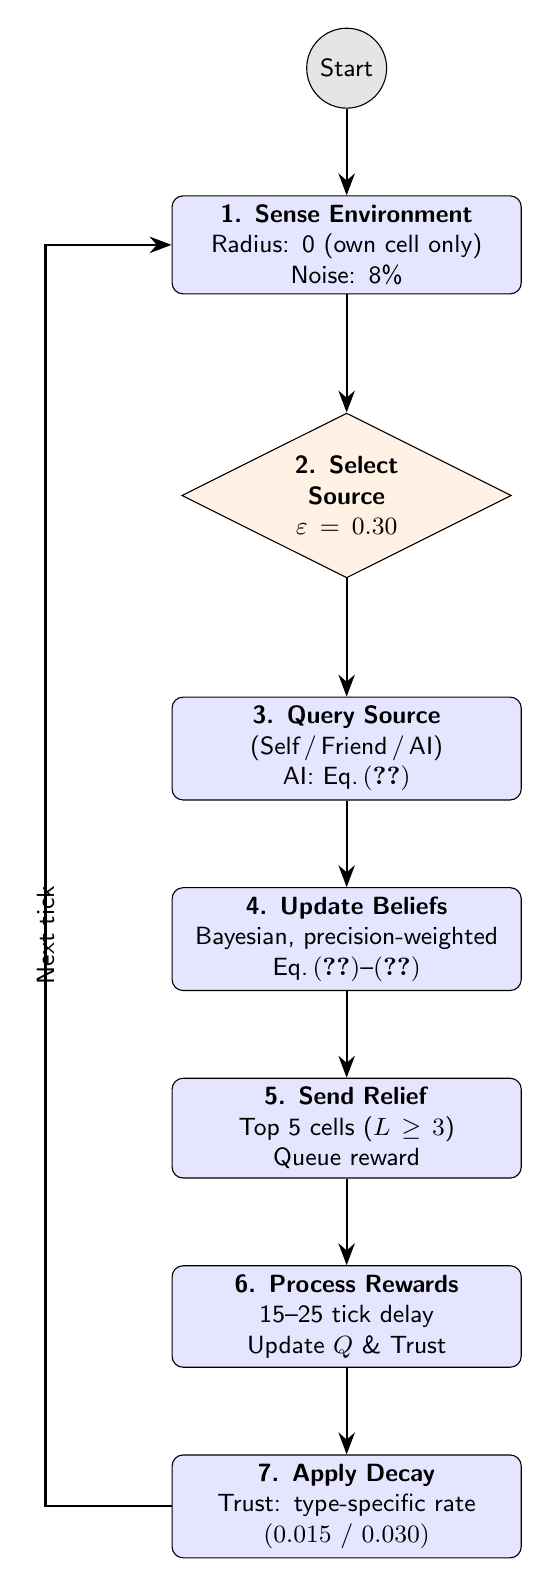
\begin{tikzpicture}[
    node distance=1.1cm and 2cm,
    every node/.style={font=\sffamily\small, align=center},
    process/.style={rectangle, draw, fill=blue!10, text width=4.2cm,
                    minimum height=1cm, rounded corners},
    decision/.style={diamond, draw, fill=orange!10, text width=2.2cm,
                     inner sep=0pt, aspect=2},
    arrow/.style={-{Stealth[scale=1.2]}, thick}
]

\node (start)  [circle, draw, fill=gray!20]                             {Start};
\node (step1)  [process, below=of start]
    {\textbf{1. Sense Environment}\\Radius: 0 (own cell only)\\Noise: 8\%};
\node (step2)  [decision, below=of step1, yshift=-0.4cm]
    {\textbf{2. Select Source}\\ $\varepsilon=0.30$};
\node (step3)  [process, below=of step2, yshift=-0.4cm]
    {\textbf{3. Query Source}\\(Self\,/\,Friend\,/\,AI)\\AI: Eq.\,\eqref{eq:alignment}};
\node (step4)  [process, below=of step3]
    {\textbf{4. Update Beliefs}\\Bayesian, precision-weighted\\Eq.\,\eqref{eq:acceptance}--\eqref{eq:bayesian}};
\node (step5)  [process, below=of step4]
    {\textbf{5. Send Relief}\\Top 5 cells ($L\!\geq\!3$)\\Queue reward};
\node (step6)  [process, below=of step5]
    {\textbf{6. Process Rewards}\\15--25 tick delay\\Update $Q$ \& Trust};
\node (step7)  [process, below=of step6]
    {\textbf{7. Apply Decay}\\Trust: type-specific rate\\$(0.015$ / $0.030)$};

\draw [arrow] (start) -- (step1);
\draw [arrow] (step1) -- (step2);
\draw [arrow] (step2) -- (step3);
\draw [arrow] (step3) -- (step4);
\draw [arrow] (step4) -- (step5);
\draw [arrow] (step5) -- (step6);
\draw [arrow] (step6) -- (step7);
\draw [arrow] (step7.west) -- ++(-1.6,0) |- (step1.west)
    node[pos=0.25, left, rotate=90] {Next tick};
\end{tikzpicture}
\caption{Per-tick decision cycle for human agents.
         Source selection uses an $\varepsilon$-greedy Q-learning strategy.
         Belief updating follows the precision-weighted Bayesian mechanism
         (Equations~\ref{eq:acceptance}--\ref{eq:bayesian}).
         Reward processing is delayed 15--25 ticks to model logistical
         pipelines; trust updates use agent-type-specific learning rates.}
\label{fig:cycle}
\end{figure}

When agents receive a report $r$ from any source, they accept it with probability
%
\begin{equation}
  P(\text{accept}) = \frac{D_{\mathrm{eff}}^{\delta}}
                          {|r-b|^{\delta}+D_{\mathrm{eff}}^{\delta}},
  \label{eq:acceptance}
\end{equation}
%
where $D_{\mathrm{eff}} = D\cdot(1+0.5\,T_{\mathrm{source}})$ for social contacts
(trust-widened) and $D_{\mathrm{eff}}=D$ for the AI.
If the report is accepted, the posterior is precision-weighted:
%
\begin{equation}
  b' = \frac{\pi_{\mathrm{prior}}\,b + \pi_{\mathrm{source}}\,r}
            {\pi_{\mathrm{prior}} + \pi_{\mathrm{source}}},
  \label{eq:bayesian}
\end{equation}
%
with $\pi\propto c/(1-c)$ (confidence odds), scaled by a type-specific factor
(1.5 for exploitative, 0.8 for exploratory) that calibrates resistance to belief
revision.
This mechanism generalises the Deffuant bounded-confidence model
\citep{deffuant2000mixing} by replacing binary thresholding with a smooth
probability curve and by coupling the effective threshold to dynamic source trust,
producing richer dynamics while remaining analytically interpretable
\citep{lorenz2017continuous}.

When selecting information sources, agents employ an $\varepsilon$-greedy strategy
($\varepsilon=0.30$) that balances exploration of unfamiliar sources with
exploitation of trusted relationships.
The social network is constructed with type-homogeneous community structure:
exploitative agents are wired predominantly within their own cluster, exploratory
agents within theirs, with no enforced cross-type edges.
This follows empirical evidence of homophily in disaster communication networks
\citep{Bruns2012,Sutton2008}.

% ============================================================
\subsection{Trust Evolution}

Trust dynamics emerge from two parallel processes: direct observation of
information accuracy and reinforcement learning based on relief outcomes.
The trust update mechanism combines immediate feedback from ground-truth comparisons
with delayed rewards from the effectiveness of relief allocation.
This dual-track approach captures both the cognitive updating of source reliability
assessments and the pragmatic evaluation of information utility for decision support.

The model uses asymmetric trust learning rates across agent types:
exploitative agents update trust slowly ($\mathrm{lr}=0.015$), consistent with
their confirmation-seeking profile; exploratory agents update more rapidly
($\mathrm{lr}=0.030$), reflecting their higher sensitivity to new evidence.
This behavioural heterogeneity produces emergent trust differentiation that
significantly influences collective performance under varying alignment conditions.

% ============================================================
\subsection{Echo Chamber Quantification}

The Social Echo Chamber Index (SECI) measures within-community belief homogeneity
relative to population-wide variance, following the approach of
\citet{cinelli2021echo}.
Because the social network is type-homogeneous, SECI is computed separately for
each connected component (community) and then averaged by agent type.
For a community with internal belief variance $V_c$ and global population variance
$V_g$:
%
\begin{equation}
  \mathrm{SECI} =
  \begin{cases}
    \displaystyle\max\!\left(-1,\;\frac{V_c - V_g}{V_g}\right)
      & V_c < V_g \quad\text{(echo chamber)}, \\[8pt]
    \displaystyle\min\!\left(+1,\;\frac{V_c - V_g}{V_{\max} - V_g}\right)
      & V_c \geq V_g \quad\text{(anti-echo)},
  \end{cases}
  \label{eq:seci}
\end{equation}
%
where $V_{\max}=5.0$ is the maximum possible variance on the $[0,5]$ severity
scale.
$\mathrm{SECI}<0$ indicates community beliefs are more homogeneous than the global
pool (echo chamber); $\mathrm{SECI}=0$ is the null; $\mathrm{SECI}>0$ indicates
the community is more internally diverse (anti-echo).
The piecewise normalisation keeps the index symmetric on $[-1,+1]$ without
assuming that the maximum possible variance equals the global variance.

Alternative formulations based on opinion fragmentation \citep{Bail2018} or
information entropy \citep{Sasahara2021} were considered; the variance-based
approach was preferred because it has a natural zero, is directly comparable across
agent types, and maps onto the precision terms in the Bayesian update
(Equation~\ref{eq:bayesian}).

The AI Echo Chamber Index (AECI) measures the fraction of information updates
that are actually absorbed from AI sources within each five-tick window:
%
\begin{equation}
  \mathrm{AECI} = \frac{\Delta q_{\mathrm{AI}}}
                       {\Delta q_{\mathrm{AI}} + \Delta q_{\mathrm{human}}},
  \label{eq:aeci}
\end{equation}
%
where $\Delta q$ counts D$\delta$-accepted updates during the window.
Unlike a simple query-count ratio, this formulation distinguishes
\emph{reliance}---AI information that passes the acceptance threshold and
revises beliefs---from mere querying, which may be rejected without effect.
High AECI signals over-dependence on a potentially confirming source, regardless
of how often human contacts are also consulted.

% ============================================================
\subsection{Relief Allocation and Performance Evaluation}

Agents allocate relief tokens to the top five cells they judge to have severity
$L\geq3$.
Exploitative agents score cells by confidence-weighted severity; exploratory agents
add an uncertainty-reduction term that rewards directing resources to cells with
high epistemic ambiguity.
Token placement effectiveness is evaluated through delayed reward signals
(15--25 ticks) that compare allocated resources against actual need distributions
at the time of delivery.

Performance metrics encompass belief accuracy (mean absolute error against ground
truth), targeting precision (fraction of tokens directed to cells with actual
severity $\geq3$), unmet critical needs (cells with severity $\geq4$ receiving zero
tokens per tick), and spatial coverage deficit (per-cell shortfall averaged near
and far from the disaster epicentre).
Together these measures capture both efficiency and equity dimensions of disaster
response, crucial for evaluating the downstream consequences of information flow.

% ============================================================
\subsection{Experimental Framework}

The study implements two core experiments and a set of sensitivity sweeps.

\paragraph{Goldilocks alignment sweep.}
The primary experiment sweeps $\alpha$ across eleven levels ($0.0,0.1,\ldots,1.0$)
with $N=20$ independent replications per level.
Replications differ in epicentre location, agent initialisation, and stochastic
shock sequences.
Optimal alignment is identified by two composite scores, both constructed over the
steady-state window (last 75 of 200 ticks) using range normalisation across the
sweep so each component contributes on a $[0,1]$ scale:
%
\begin{align}
  \text{total\_bubble}(\alpha)
    &= |\mathrm{SECI}|_{\mathrm{norm}}(\alpha)
       + |\mathrm{AECI}|_{\mathrm{norm}}(\alpha), \label{eq:bubble}\\
  \text{total\_score}(\alpha)
    &= |\mathrm{SECI}|_{\mathrm{norm}}(\alpha)
       + |\mathrm{AECI}|_{\mathrm{norm}}(\alpha)
       + \mathrm{MAE}_{\mathrm{norm}}(\alpha). \label{eq:score}
\end{align}
%
The Goldilocks optimum $\alpha^*$ minimises total\_bubble; $\alpha^*(+\mathrm{MAE})$
minimises total\_score.
Reporting both criteria makes the trade-off between echo-chamber suppression and
belief accuracy explicit.

\paragraph{Cognitive gap sweep.}
A secondary experiment varies the cognitive gap scalar $g\in\{0.0,0.5,1.0,1.5\}$,
which scales the divergence between exploitative and exploratory acceptance
parameters from a shared midpoint while preserving their ordinal relationship
($D_{\mathrm{exploit}}<D_{\mathrm{explor}}$,
$\delta_{\mathrm{exploit}}>\delta_{\mathrm{explor}}$).
At $g=0$ both types are cognitively identical, providing a null condition for
heterogeneity effects; $g=1$ recovers the baseline calibration
(Table~\ref{tab:S4}).
This sweep tests whether $\alpha^*$ is robust to within-population cognitive
diversity.

\paragraph{Factor sensitivity sweeps.}
One-at-a-time sweeps over agent-type composition, disaster dynamics, and rumour
probability (detailed in Table~\ref{tab:S8}) test the generalisability of the
Goldilocks finding across environmental and population variation.

Statistical analysis employs non-parametric methods to handle non-normal
performance distributions across the 20 replications, while time-series analysis
tracks the evolution of trust and bubble metrics throughout each crisis scenario.
Spatial and network periphery analyses decompose outcomes by distance to the
disaster epicentre (nearest vs.\ furthest quartile of cells) and by social-network
degree (Q1 vs.\ Q4 agents) to examine whether alignment benefits are equitably
distributed.

% ============================================================
\subsection{Technical Implementation}

The model is implemented in Python~3.11 using the Mesa~3.x framework for agent
scheduling, NetworkX for community detection and social-network analysis, and
NumPy / Matplotlib for computation and visualisation.
All simulation runs are seeded via \texttt{numpy.random.seed(run\_index)},
ensuring bit-for-bit reproducibility.
Results are serialised to JSON after each $(\alpha, \text{run})$ cell; the
plotting pipeline reads these files without re-running the simulation, so all
figures can be regenerated without recomputation.
Full parameter tables and software dependencies are provided in the supplementary
materials (Tables~S1--S2, S9).




\section{Discussion}\label{sec12}

Discussions should be brief and focused. In some disciplines use of Discussion or `Conclusion' is interchangeable. It is not mandatory to use both. Some journals prefer a section `Results and Discussion' followed by a section `Conclusion'. Please refer to Journal-level guidance for any specific requirements. 

\section{Conclusion}\label{sec13}

Conclusions may be used to restate your hypothesis or research question, restate your major findings, explain the relevance and the added value of your work, highlight any limitations of your study, describe future directions for research and recommendations. 

In some disciplines use of Discussion or 'Conclusion' is interchangeable. It is not mandatory to use both. Please refer to Journal-level guidance for any specific requirements. 

\backmatter

\bmhead{Supplementary information}

If your article has accompanying supplementary file/s please state so here. 

Authors reporting data from electrophoretic gels and blots should supply the full unprocessed scans for key as part of their Supplementary information. This may be requested by the editorial team/s if it is missing.

Please refer to Journal-level guidance for any specific requirements.

\bmhead{Acknowledgements}

Acknowledgements are not compulsory. Where included they should be brief. Grant or contribution numbers may be acknowledged.

Please refer to Journal-level guidance for any specific requirements.

\section*{Declarations}

Some journals require declarations to be submitted in a standardised format. Please check the Instructions for Authors of the journal to which you are submitting to see if you need to complete this section. If yes, your manuscript must contain the following sections under the heading `Declarations':

\begin{itemize}
\item Funding
\item Conflict of interest/Competing interests (check journal-specific guidelines for which heading to use)
\item Ethics approval and consent to participate
\item Consent for publication
\item Data availability 
\item Materials availability
\item Code availability 
\item Author contribution
\end{itemize}

\noindent
If any of the sections are not relevant to your manuscript, please include the heading and write `Not applicable' for that section. 

%%===================================================%%
%% For presentation purpose, we have included        %%
%% \bigskip command. Please ignore this.             %%
%%===================================================%%
\bigskip
\begin{flushleft}%
Editorial Policies for:

\bigskip\noindent
Springer journals and proceedings: \url{https://www.springer.com/gp/editorial-policies}

\bigskip\noindent
Nature Portfolio journals: \url{https://www.nature.com/nature-research/editorial-policies}

\bigskip\noindent
\textit{Scientific Reports}: \url{https://www.nature.com/srep/journal-policies/editorial-policies}

\bigskip\noindent
BMC journals: \url{https://www.biomedcentral.com/getpublished/editorial-policies}
\end{flushleft}

\begin{appendices}


\bibliography{References}

\newpage

\section*{Supplementary Materials}
%\addcontentsline{toc}{section}{Supplementary Materials}

% Renumber tables and figures with S prefix
\renewcommand{\thetable}{S\arabic{table}}
\renewcommand{\thefigure}{S\arabic{figure}}
\renewcommand{\theequation}{S\arabic{equation}}
\setcounter{table}{0}
\setcounter{figure}{0}
\setcounter{equation}{0}

% ============================================================
\subsection*{S1\quad Model Parameters}

\begin{table}[h]
\centering
\caption{Fixed simulation parameters (all experiments).}
\label{tab:S1}
\small
\begin{tabular}{llll}
\toprule
Parameter & Symbol & Value & Rationale \\
\midrule
Grid width / height         & ---  & $30\times30$   & Sufficient spatial resolution; tractable for $N=20$ replications \\
Number of human agents      & $N$  & 100            & Large enough for network effects; small enough to track individually \\
AI agents                   & ---  & 5              & $\approx$1 AI per 20 humans; non-negligible but not dominant coverage \\
AI sensing fraction (per tick) & ---& 0.15          & AI observes 15\% of the 900-cell grid ($\approx$135 cells/tick) \\
Share of exploitative agents & ---  & 0.50          & Balanced population; varied in factor sweep (Table~\ref{tab:S8}) \\
Share of confirming social ties & --- & 0.70        & Reflects documented homophily in disaster communication \\
Disaster dynamics mode      & ---  & 2              & Medium-tempo: cells drift $\pm1$--$2$ levels/tick toward baseline \\
Shock probability (per cell/tick) & --- & 0.10      & Persistent environmental non-stationarity \\
Shock magnitude             & ---  & $\pm2$ levels  & Produces salient deviations requiring active information-seeking \\
Simulation length           & $T$  & 200 ticks      & Allows learning, echo-chamber formation, and steady-state measurement \\
Initial (human) trust       & ---  & 0.30           & Low baseline prevents unrealistic blind trust at $t=0$ \\
Initial AI trust            & ---  & 0.25           & Slight AI scepticism, consistent with survey findings \\
Q-learning rate             & $\eta$ & 0.10         & Standard value; sensitivity analysis unreported \\
$\varepsilon$-greedy exploration & $\varepsilon$ & 0.30 & Ensures continued source diversity throughout run \\
Trust learning rate (exploitative) & --- & 0.015   & Slow trust revision matches confirmation-seeking profile \\
Trust learning rate (exploratory)  & --- & 0.030   & Faster but still sub-linear trust revision \\
Rumour probability          & ---  & 1.00           & All social information propagated (worst-case echo scenario) \\
Relief outcome delay        & ---  & 15--25 ticks   & Random; models logistical pipeline in humanitarian response \\
Steady-state window         & ---  & 75 ticks       & Last 75 of 200 ticks (15 samples at the 5-tick cadence) \\
\bottomrule
\end{tabular}
\end{table}

% ============================================================
\subsection*{S2\quad Agent Cognitive Parameters}

\begin{table}[h]
\centering
\caption{Bayesian acceptance parameters by agent type.}
\label{tab:S2}
\small
\begin{tabular}{llll}
\toprule
Parameter & Exploitative & Exploratory & Interpretation \\
\midrule
Acceptance half-width, $D$   & 2.0 & 4.0 & Distance at which $P(\text{accept})=0.5$ \\
Acceptance steepness, $\delta$ & 3.5 & 1.2 & Higher $\delta$ $\Rightarrow$ sharper threshold \\
Precision weight             & $1.5\times c/(1-c)$ & $0.8\times c/(1-c)$ & Resistance to belief revision ($c$ = confidence) \\
Sensing radius               & 0 cells & 0 cells & Both types rely on communication \\
Interest-point targeting     & Believed epicentre & Highest-uncertainty cell & Governs query direction \\
\bottomrule
\end{tabular}
\end{table}

The acceptance probability for report $r$ given prior belief $b$ is
%
\begin{equation}
  P(\text{accept}) = \frac{D_{\mathrm{eff}}^{\delta}}{|r-b|^{\delta}+D_{\mathrm{eff}}^{\delta}},
  \tag{S1}
\end{equation}
%
where $D_{\mathrm{eff}} = D\cdot(1+0.5\,T_{\mathrm{source}})$ for social
contacts and $D_{\mathrm{eff}}=D$ for the AI.
This generalises the bounded-confidence model of \citet{Deffuant2000} by
replacing the binary threshold with a smooth curve parameterised by $(D,\delta)$.

% ============================================================
\subsection*{S3\quad AI Alignment Mechanism}

The AI response formula is
%
\begin{equation}
  r_{\mathrm{AI}} = (1-\alpha)\,t + \alpha\,b,
  \tag{S2}
\end{equation}
%
where $t$ is the ground-truth cell severity, $b$ is the querying agent's current
belief, and $\alpha\in[0,1]$ is the alignment parameter.
At $\alpha=0$: $r_{\mathrm{AI}}=t$ (fully truthful).
At $\alpha=1$: $r_{\mathrm{AI}}=b$ (perfect confirmation).
Intermediate values produce a weighted average --- the AI is partially informative
and partially sycophantic.

This linear interpolation is the simplest formulation spanning the
truth--confirmation spectrum without additional free parameters.
Non-linear or stochastic variants (e.g.\
$r\sim\mathcal{N}(\alpha b+(1-\alpha)t,\,\sigma^2)$) were not pursued in the
main sweep to preserve interpretability; adding symmetric noise shifts all
SECI/AECI curves uniformly without displacing $\alpha^*$.

% ============================================================
\subsection*{S4\quad Cognitive Gap Scalar}

The gap scalar $g$ parameterises cognitive divergence between agent types around
a shared midpoint:
%
\begin{align}
  D_{\mathrm{exploit}}(g) &= \max(3.0 - 1.0\,g,\;0.1),
  &\delta_{\mathrm{exploit}}(g) &= 2.35 + 1.15\,g, \tag{S3}\\
  D_{\mathrm{explor}}(g)  &= 3.0 + 1.0\,g,
  &\delta_{\mathrm{explor}}(g)  &= \max(2.35 - 1.15\,g,\;0.1). \tag{S4}
\end{align}

\begin{table}[h]
\centering
\caption{Cognitive parameters at each gap-scalar value.}
\label{tab:S4}
\begin{tabular}{ccccc}
\toprule
$g$ & $D_{\mathrm{exploit}}$ & $\delta_{\mathrm{exploit}}$ & $D_{\mathrm{explor}}$ & $\delta_{\mathrm{explor}}$ \\
\midrule
0.0 & 3.00 & 2.35 & 3.00 & 2.35 \\
0.5 & 2.50 & 2.93 & 3.50 & 1.78 \\
1.0 & 2.00 & 3.50 & 4.00 & 1.20 \\
1.5 & 1.50 & 4.08 & 4.50 & 0.63 \\
\bottomrule
\end{tabular}
\end{table}

The shared midpoint ($D_{\mathrm{mid}}=3.0$, $\delta_{\mathrm{mid}}=2.35$) is
the arithmetic mean of the baseline exploit/explor values.
At $g=0$ both types are cognitively identical, providing a null condition for
heterogeneity effects.
The invariant $D_{\mathrm{exploit}}<D_{\mathrm{explor}}$ and
$\delta_{\mathrm{exploit}}>\delta_{\mathrm{explor}}$ holds for all $g>0$,
ensuring the exploitative type always has a narrower and steeper acceptance curve.

The gap sweep uses $N=2$ replications per $(g,\alpha)$ cell and runs for
$\max(50,T/2)=125$ ticks.
This differs from the primary sweep ($N=20$, $T=200$); results are therefore
interpreted as indicative rather than confirmatory.

% ============================================================
\subsection*{S5\quad Metric Definitions}

\subsubsection*{S5.1\enspace Social Echo Chamber Index (SECI)}

\begin{equation}
  \mathrm{SECI} = 1 -
    \frac{\mathrm{Var}\!\bigl(\{b_{f,k}:f\in\mathrm{friends}(i),\,k\in\mathcal{K}\}\bigr)}
         {\mathrm{Var}\!\bigl(\{b_{j,k}:j\in\mathcal{A},\,k\in\mathcal{K}\}\bigr)},
  \tag{S5}
\end{equation}
%
where $\mathcal{A}$ is the set of all agents and $\mathcal{K}$ is the set of all
grid cells.
Computed separately for exploitative and exploratory agents every five ticks.
A \emph{formation} event is registered when $\mathrm{SECI}<-0.30$ sustained for
$\geq3$ consecutive samples; a \emph{recovery} event when
$\mathrm{SECI}\geq0.0$ sustained for $\geq5$ consecutive samples after formation.
If formation never occurs the lifecycle bar is left blank ($\circ$); if formation
occurs but recovery does not before the run ends the bar reaches maximum height
with annotation $\times$.

\subsubsection*{S5.2\enspace AI Echo Chamber Index (AECI)}

\begin{equation}
  \mathrm{AECI} = \frac{\Delta q_{\mathrm{AI}}}
                       {\Delta q_{\mathrm{AI}} + \Delta q_{\mathrm{human}}},
  \tag{S6}
\end{equation}
%
where $\Delta q$ denotes the increment in \emph{accepted} information-update
calls over a five-tick window.
This window-delta formulation distinguishes recent reliance from cumulative
history, making AECI responsive to within-run behavioural shifts.

\subsubsection*{S5.3\enspace Belief Accuracy (MAE)}

\begin{equation}
  \mathrm{MAE} = \frac{1}{|\mathcal{C}|}\sum_{k\in\mathcal{C}}|b_{i,k}-t_k|,
  \tag{S7}
\end{equation}
%
averaged over agents $i$, where $\mathcal{C}=\{k:t_k\geq1\}$ is the set of
cells with non-zero true severity.

\subsubsection*{S5.4\enspace Composite Goldilocks Scores}

Let $\bar{m}(\alpha)$ denote the steady-state mean (last 75 ticks) of metric $m$
at alignment level $\alpha$.
Range normalisation across the sweep:
%
\begin{equation}
  m_{\mathrm{norm}}(\alpha) =
    \frac{\bar{m}(\alpha)-\min_{\alpha}\bar{m}}
         {\max_{\alpha}\bar{m}-\min_{\alpha}\bar{m}}.
  \tag{S8}
\end{equation}
%
Composite scores:
%
\begin{align}
  \text{total\_bubble}_{\mathrm{norm}}(\alpha)
    &= |\mathrm{SECI}|_{\mathrm{norm}}(\alpha)
       +|\mathrm{AECI}|_{\mathrm{norm}}(\alpha), \tag{S9}\\
  \text{total\_score}_{\mathrm{norm}}(\alpha)
    &= |\mathrm{SECI}|_{\mathrm{norm}}(\alpha)
       +|\mathrm{AECI}|_{\mathrm{norm}}(\alpha)
       +\mathrm{MAE}_{\mathrm{norm}}(\alpha). \tag{S10}
\end{align}
%
Optima:
%
\begin{align}
  \alpha^* &= \arg\min_{\alpha}\,\text{total\_bubble}_{\mathrm{norm}}(\alpha), \tag{S11}\\
  \alpha^*(+\mathrm{MAE}) &= \arg\min_{\alpha}\,\text{total\_score}_{\mathrm{norm}}(\alpha). \tag{S12}
\end{align}
%
Range normalisation ensures each component contributes on the same $[0,1]$ scale
regardless of the absolute magnitude of SECI, AECI, or MAE.
The two optima are reported separately so that the trade-off between
echo-chamber suppression and accuracy improvement is explicit.

\subsubsection*{S5.5\enspace Spatial and Network Periphery Metrics}

\paragraph{Spatial periphery.}
For each simulation run, cells are ranked by Euclidean distance to that run's
epicentre.
\emph{Near} cells (Q1, closest quartile) and \emph{far} cells (Q4, furthest
quartile) are identified per run; coverage deficit (actual severity minus mean
aid tokens per tick) and aid density are averaged within each set and then
averaged across replications.
This per-run computation avoids the blurring artefact that would arise from
projecting all replications onto a single grid when epicentre locations vary.

\paragraph{Network periphery.}
Agents are ranked by social-network degree.
Low-degree agents (Q1) and high-degree agents (Q4) are compared on belief MAE
and relief tokens sent per tick.

% ============================================================
\subsection*{S6\quad Primary Experiment: Goldilocks Alignment Sweep}

\begin{table}[h]
\centering
\caption{Experiment design: primary Goldilocks alignment sweep.}
\label{tab:S6}
\begin{tabular}{lll}
\toprule
Dimension & Values & $N$ per cell \\
\midrule
AI alignment $\alpha$
  & $0.0,\,0.1,\,0.2,\ldots,1.0$ (11 levels) & 20 \\
Agent type mix
  & 50\% exploit\,/\,50\% explor (fixed) & --- \\
Simulation length $T$
  & 200 ticks & --- \\
\midrule
\textbf{Total simulation runs} & \multicolumn{2}{l}{\textbf{220}} \\
\bottomrule
\end{tabular}
\end{table}

Each replication uses an independent random seed for epicentre placement, agent
initialisation, and shock sequences.
Results are presented as boxplots (median, IQR, $1.5\times$IQR whiskers) over the
20 replications.
Steady-state scalars are averaged over the last 75 ticks (15 samples at the
5-tick cadence).

% ============================================================
\subsection*{S7\quad Secondary Experiment: Cognitive Gap Sweep}

\begin{table}[h]
\centering
\caption{Experiment design: cognitive gap sweep.}
\label{tab:S7}
\begin{tabular}{lll}
\toprule
Dimension & Values & $N$ per cell \\
\midrule
Gap scalar $g$               & $\{0.0,\,0.5,\,1.0,\,1.5\}$        & 2 \\
AI alignment $\alpha$ (within each $g$)
                             & $0.0,\,0.1,\ldots,1.0$ (11 levels)  & 2 \\
Simulation length $T$        & 125 ticks ($=\max(50,200/2)$)        & --- \\
\midrule
\textbf{Total simulation runs} & \multicolumn{2}{l}{\textbf{88}} \\
\bottomrule
\end{tabular}
\end{table}

The shortened run length and reduced replication count are intentional: the gap
sweep is a parameter-sensitivity check rather than a primary confirmatory
analysis.
Both $\alpha^*(\text{bubble})$ and $\alpha^*(+\mathrm{MAE})$ are computed for
each $g$ level and plotted as grouped bars.
Absolute (non-normalised) composite scores are shown to allow cross-$g$
comparison; normalised scores within each $g$ sweep would confound changes in
magnitude with changes in the optimal $\alpha$.

% ============================================================
\subsection*{S8\quad Factor Sensitivity Sweeps}

Three one-at-a-time factor sweeps test the robustness of the Goldilocks finding.
All use $\alpha=0.5$ and $N=2$ replications with run length
$\max(50,T/2)=125$ ticks.

\begin{table}[h]
\centering
\caption{Factor sensitivity sweep design.}
\label{tab:S8}
\begin{tabular}{lll}
\toprule
Factor & Values swept & Fixed parameters \\
\midrule
Share of exploitative agents & $\{0.2,\,0.5,\,0.8\}$
  & All base parameters except \texttt{share\_exploitative} \\
Disaster dynamics mode & $\{0,\,2,\,3\}$
  & All base parameters except \texttt{disaster\_dynamics} \\
Rumour probability & $\{0.0,\,0.5,\,1.0\}$
  & All base parameters except \texttt{rumor\_probability} \\
\bottomrule
\end{tabular}
\end{table}

Disaster dynamics mode controls the rate at which cell severities drift and
receive shocks: mode~0 fixes the initial map; mode~2 applies the baseline shock
schedule (Table~\ref{tab:S1}); mode~3 doubles shock frequency.

% ============================================================
\subsection*{S9\quad Software and Reproducibility}

The model is implemented in Python~3.11 using Mesa~3.x for agent scheduling,
NetworkX for social-network construction, and NumPy / Matplotlib for numerical
computation and visualisation.
All simulation runs are seeded via \texttt{numpy.random.seed(run\_index)},
ensuring bit-for-bit reproducibility given the same Python and library versions.
Results are serialised to JSON after each $(\alpha,\mathrm{run})$ cell; the
plotting pipeline reads these files without re-running the simulation, so figures
can be regenerated without recomputation.

\begin{table}[h]
\centering
\caption{Software dependencies.}
\label{tab:S9}
\begin{tabular}{ll}
\toprule
Package & Version \\
\midrule
Python     & 3.11 \\
Mesa       & $\geq$3.0 \\
NetworkX   & $\geq$3.0 \\
NumPy      & $\geq$1.24 \\
Matplotlib & $\geq$3.7 \\
SciPy      & $\geq$1.10 \\
\bottomrule
\end{tabular}
\end{table}

The full codebase is available at the repository listed on the title page.
Raw JSON result files for the main sweep ($N=20$) require approximately 150~MB
of disk space and are archived separately

\end{appendices}

%%===========================================================================================%%
%% If you are submitting to one of the Nature Portfolio journals, using the eJP submission   %%
%% system, please include the references within the manuscript file itself. You may do this  %%
%% by copying the reference list from your .bbl file, paste it into the main manuscript .tex %%
%% file, and delete the associated \verb+\bibliography+ commands.                            %%
%%===========================================================================================%%



\end{document}
